\subsection{Tracking}

In order to measure a vehicle's speed and position it is necessary to track its position over time. Each vehicle object's location in an image is represented by the center of its bounding box called a centroid and by maintaining a history of an object's centroid position over time its path can be tracked through the video. For each image new centroids are recalculated for every object, by comparing the new centroid locations with the old centroid locations an educated guess can be made about the new position of the objects. New centroids are assigned to the objects whose last known position was closest. If a new position cannot be found for an object then it has a limited number of frames it can be missing for before it's removed, objects generally go missing due to partial or complete occlusion by other vehicles, alternatively they will go missing permanently if they leave the node's field of view. Vehicle's can also disappear if they remain stationery long enough to be considered background pixels by the subtractor. Figure \ref{fig:centroids} visualizes the centroids on the objects along with a unique identifier which is used to mark ownership of a foreground object. The implementation of the tracking design was based heavily on the work of Adrian Rosebrock as outlined in his tutorial series on PyImageSearch \cite{adrian_rosebrock_simple_object_tracking}. Notice in Figure \ref{fig:centroids} centroids 25 and 24 belong to no object, this is because they have not yet timed out, meaning their object hasn't been missing from frame long enough for them to be dismissed, this is also the case for centroid 16. Centroids 1 and 9 belong to a cluster of vehicles that have become distant (see Figure \ref{fig:original_frame}), this occurs because as the vehicles travel further away the distance between them in pixels becomes less and so the morphological process presses them together. This is not an issue if the counting and measuring system is calibrated to focus on areas where vehicles are easily separable.

\begin{figure}[H]
    \centering
    \centering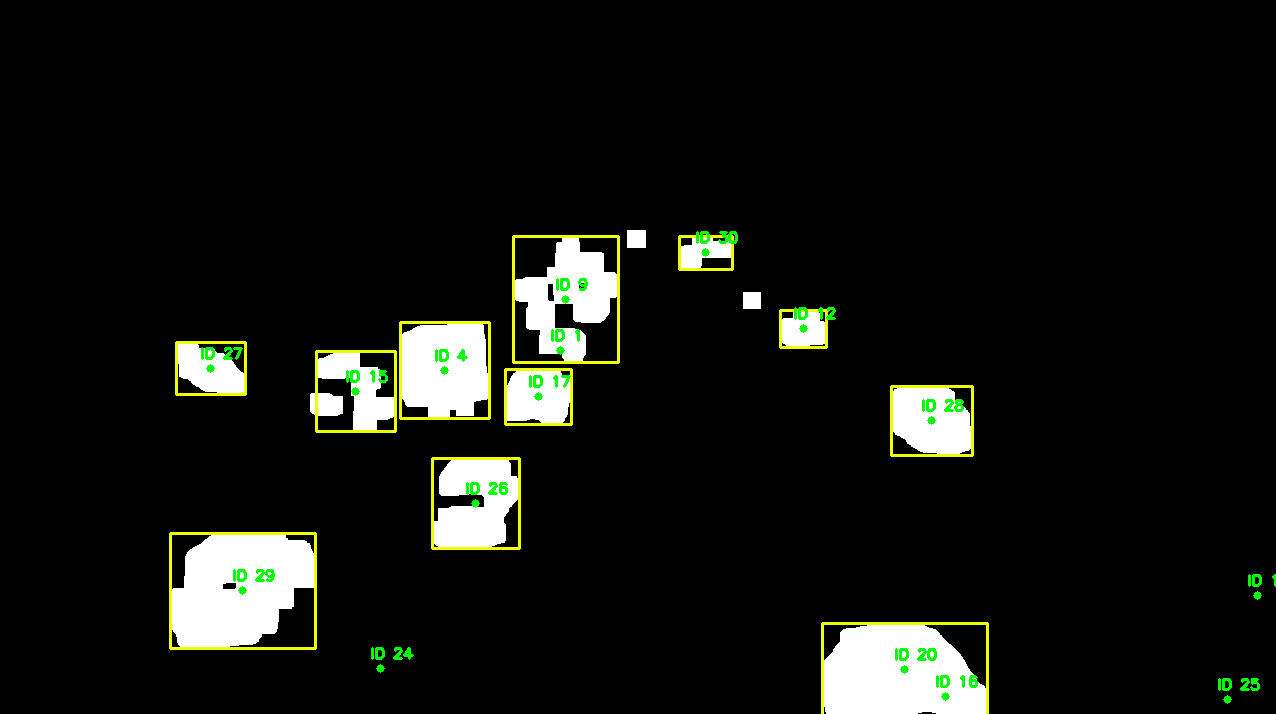
\includegraphics[width = 0.8\textwidth]{design/detection/tracking/mask_centroids}
    \caption{Centroids plotted over foreground objects.}
    \label{fig:centroids}
\end{figure}

\subsubsection{Calibration}

Centroid tracking is critical to vehicle count and speed estimation and so any centroid that doesn't represented a vehicle will distort the results of the system therefore tracking must be calibrated to produce the best results possible. We seek to calibrate the tracking for a specific region the image where centroids are most consistently found there will always be, however, centroids that don't belong to true vehicles but fractured parts of them that didn't become connected during morphology. The false centroids are handled by consolidating them into a single centroid based on their proximity to each other. The assumption is that for a given vehicle scale in a specified region no vehicles can be closer together than the minimum width used to assign contours and so if two or more centroids are closer than this threshold they are combined into one. The specific combination threshold distance can be guided by the bounding box threshold dimensions and visual analysis the output of the system. Figure \ref{fig:centroids_consolidation} compares two centroid allocations for the same image where one perform centroid combination and the other doesn't. In Figure \ref{fig:consolidateA} the number of centroids is greater thus consuming more computational power and increasing the number of false positive counts. 

The second calibration consideration for tracking is how long the system remembers an object for after it goes missing. Determination of how long a centroid should be stored while missing is dependent on how frequently vehicles are occluded and for how long. In a situation where there was an obstacle consistently blocking vision of the road for a period then the amount of time a centroid should be stored is proportional to how long a vehicle is occluded by that obstacle on average. If a vehicle's centroid is dismissed prematurely it is not terribly disruptive so long as the vehicle is recognised again before it is counted though it may affect whether or not that vehicle's speed is recorded as a certain history length is required to do so. 

\begin{figure}[H]
\centering
\begin{subfigure}[b]{0.45\linewidth}
            \centering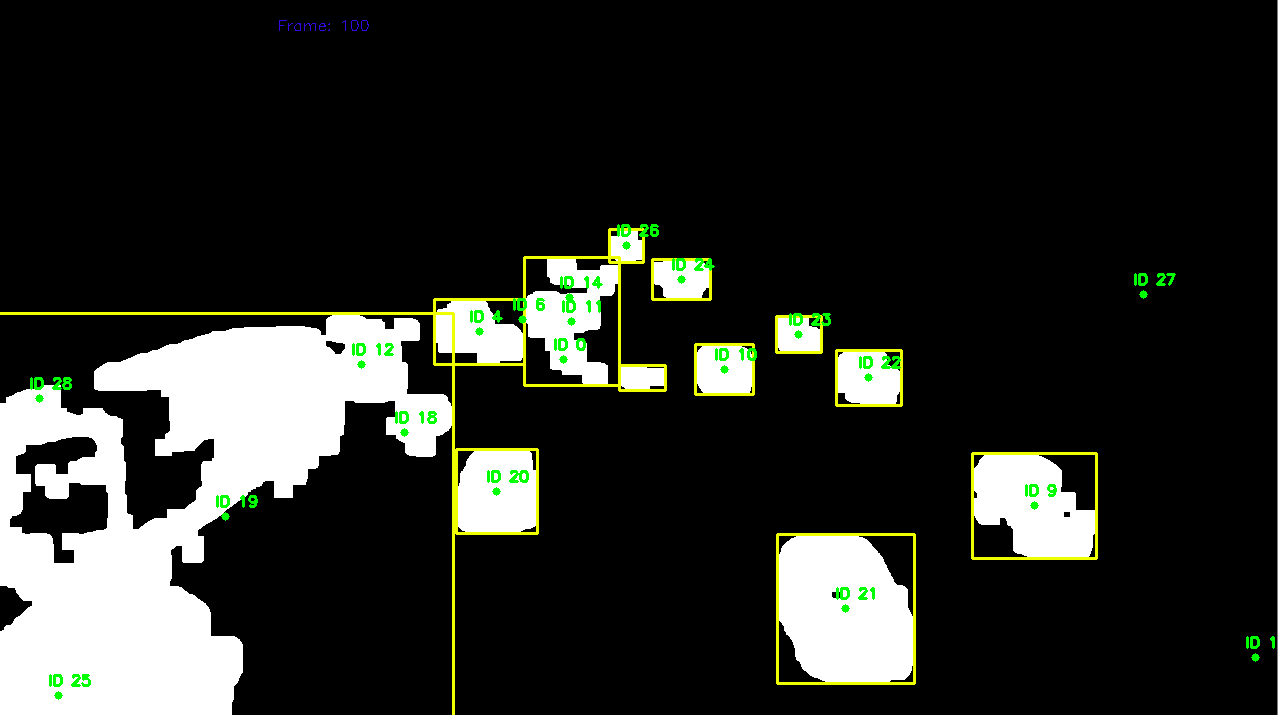
\includegraphics[width = \textwidth]{design/detection/calibration/mask_noconsolidate}
            \captionsetup{format=hang}
            \caption{Centroid tracking with no consolidation distance set (16 centroids).}
            \label{fig:consolidateA}
  \label{fig:}
    \end{subfigure}
    \begin{subfigure}[b]{0.45\linewidth}
            \centering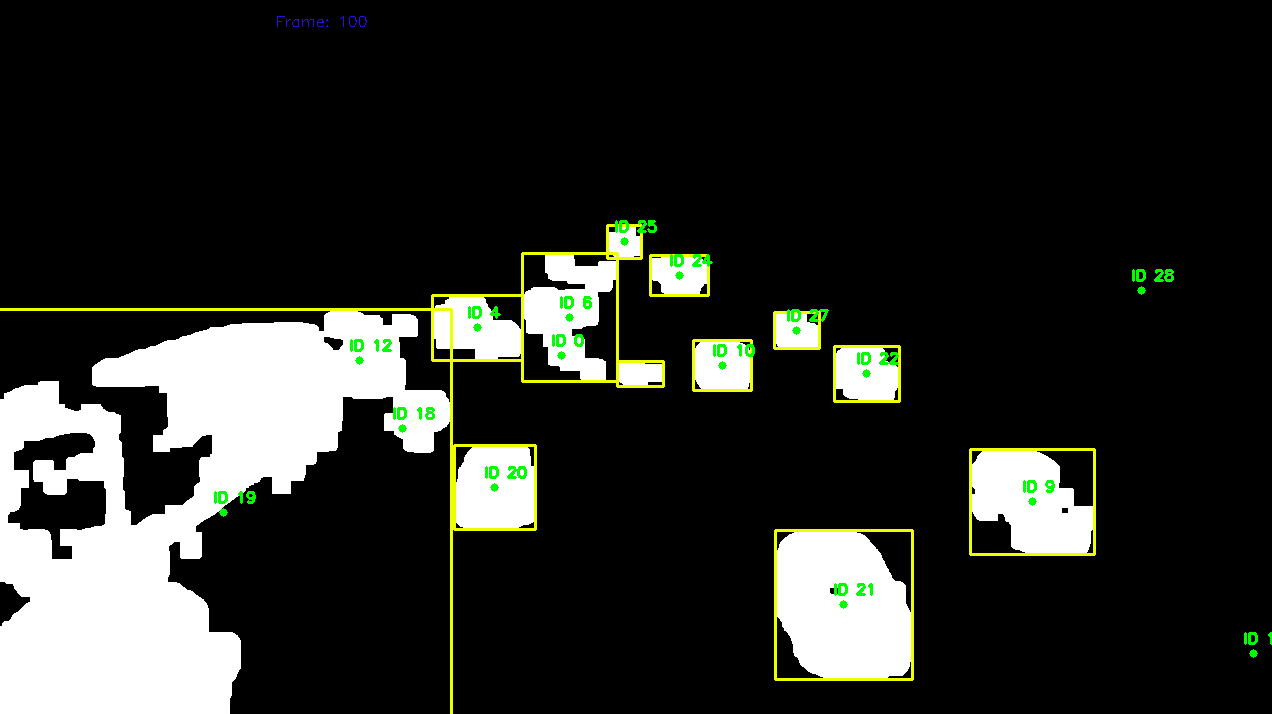
\includegraphics[width = \textwidth]{design/detection/calibration/mask_consolidate}
            \captionsetup{format=hang}
        \caption{Centroid tracking with consolidation distance set (20 centroids).}
        \label{fig:consolidateB}
      \end{subfigure}
      \captionsetup{format=hang}
    \caption{Comparison of centroid generation with and without consolidating centroids based on distance.}
    \label{fig:centroids_consolidation}
\end{figure}
  
